\documentclass[logo,reportComp]{thesis}
\usepackage[cpp,pseudo]{mypackage}

\title{操作系统原理实验报告}
\subtitle{实验八:进程同步与信号量机制}
\school{数据科学与计算机学院}
\author{陈鸿峥}
\classname{17大数据与人工智能}
\stunum{17341015}
\headercontext{操作系统原理实验报告}
% \authorremark{本实验报告用\LaTeX撰写,创建时间:\builddate\today}

\begin{document}

\maketitle

\section{实验目的}
\begin{itemize}
	\item 学习信号量机制的原理,掌握其实现方法。
	\item 利用信号量机制,实现进程互斥和同步,理解并发进程的同步与互斥原理。
	\item 扩展MyOS,实现信号量机制。
\end{itemize}

\section{实验要求}
% 实验目的和实验要求由老师提供实验项目文档中获取
如果内核实现了信号量机制相关的系统调用,并在c库中封装相关的系统调用,那么,我们的c语言就也可以实现多进程同步的应用程序了。

例如:利用进程控制操作,父进程f创建二个子进程s和d,大儿子进程s反复向父进程f祝福,小儿子进程d反复向父进程送水果(每次一个苹果或其他水果),当二个子进程分别将一个祝福写到共享数据a和一个水果放进果盘后,父进程才去享受:从数组a收取出一个祝福和吃一个水果,如此反复进行。
\begin{enumerate}
	\item 适当增加操作时延,观察和捕捉RC问题,截屏并说明。
	\item 利用信号量和PV操作协调进程的并发
\end{enumerate}
% 在实验五或更后的原型基础上,进化你的原型操作系统,原型保留原有特征的基础上,设计满足下列要求的新原型操作系统:
% (1)在内核实现信号量机制,定义100个可用信号量,并以系统调用的方式实现初始化init()、p()和v()三个基本操作。
% (2)内核实现信号量机制后,在c库中封装相关的系统调用.
% (3)编写一个c语言程序,实现有限缓冲的生产者-消费者模型的应用程序。
% 编译连接你编写的用户程序,产生一个com文件,放进程原型操作系统映像盘中。

\section{实验环境}
% 包括:硬件或虚拟机配置方法、软件工具与作用、方案的思想、相关原理、程序流程、算法和数据结构、程序关键模块,结合代码与程序中的位置进行解释。不得抄袭,否则按作弊处理。
% 实验方案包括相关基础原理、实验工具和环境、程序流程和算法思想、数据结构与程序模块功能说明,代码文档组成说明等
具体环境选择原因已在实验一报告中说明。
\begin{itemize}
	\item Windows 10系统 + Ubuntu 18.04(LTS)子系统
	\item gcc 7.3.0 + nasm 2.13.02 + GNU ld (Binutils) 2.3.0
	\item GNU Make 4.1
	\item Oracle VM VirtualBox 6.0.6
	\item Bochs 2.6.9
	\item Sublime Text 3 + Visual Studio Code 1.33.1
\end{itemize}

虚拟机配置:内存4M,1.44M虚拟软盘引导,1.44M虚拟硬盘。

\section{实验方案}
% 包括:主要工具安装使用过程及截图结果、程序过程中的操作步骤、测试数据、输入及输出说明、遇到的问题及解决情况、关键功能或操作的截图结果。不得抄袭,否则按作弊处理。
{\textbf{\textcolor{red}{本次实验继续沿用实验六保护模式的操作系统。}}}

本节所讲的内容基本都在\verb'semaphore.h'头文件中实现。

\subsection{信号量的定义}
信号量即一个整数和一个指针组成的结构体,整数是信号量的值,指针指向该信号量的进程队列。
\begin{lstlisting}
typedef struct Semaphore {
    int val;
    bool used;
    process* head;
} Semaphore;
\end{lstlisting}

由于有多个信号量,为方便管理,故添加了一个布尔类型\verb'used',用以判断该信号量是否被使用。
进而可以用一个数组来存储所有的信号量。
\begin{lstlisting}
Semaphore sem_list[N_SEMAPHORE];
\end{lstlisting}

\subsection{初始化信号量}
这部分内容实施在\verb'sem_init'中,即对每一信号量的\verb'used'位置0,并将阻塞队列置空。

\subsection{获取及释放信号量}
对信号量数组进行遍历,若某一信号量未被使用,则进行初始化,并返回其索引。
其中参数\verb'val'为信号量的初始值。
\begin{lstlisting}
int do_getsem(int val) {
    for(int i = 0; i < N_SEMAPHORE; ++i) {
        if(!sem_list[i].used) {
            sem_list[i].val = val;
            sem_list[i].used = true;
            return i;
        }
    }
    return -1;
}
\end{lstlisting}

释放信号量则更为简单,直接将其\verb'used'位置0即可,同时头指针指空。
\begin{lstlisting}
void do_freesem(int sem_id) {
    sem_list[sem_id].used = false;
    sem_list[sem_id].head = NULL;
}
\end{lstlisting}

\subsection{P操作}
P操作或者称\verb'semWait',即对信号量的值减1。
如果信号量的值\textbf{小于0},则阻塞当前进程。

为实现阻塞队列,我在原\verb'process'结构体中添加了\verb'process* next'的成员,用于构建阻塞链表。
当当前进程需要被阻塞时,将当前进程的链表指针指向该信号量阻塞队列的头部,然后将信号量的阻塞队列指针指向当前进程。
这里的调度策略是类似栈的FILO策略,因为每次都插入在链表头部,这可以大大避免遍历链表的开销,但可能造成某些进程的执行次数较少。

注意要保证P操作的原子性,这里采用了不那么优美的关中断方法,同样能实现操作。
\begin{lstlisting}
void do_sem_p(int sem_id) { // sem_wait
    disable();
    sem_list[sem_id].val--;
    if (sem_list[sem_id].val < 0) {
        curr_proc->next = sem_list[sem_id].head;
        sem_list[sem_id].head = curr_proc;
        do_wait();
    }
    enable();
}
\end{lstlisting}

\subsection{V操作}
V操作或者称\verb'semSignal',即对信号量的值加1。
如果信号量的值\textbf{小于等于0},则唤醒一阻塞进程。

唤醒进程直接从阻塞队列头部获取即可,然后将队列指针向后移一位,即实现阻塞队列的缩减。

同样要注意保证V操作的原子性,需要进行关中断。
\begin{lstlisting}
void do_sem_v(int sem_id) { // sem_signal
    disable();
    sem_list[sem_id].val++;
    if (sem_list[sem_id].val <= 0) {
        int pid = sem_list[sem_id].head->pid;
        sem_list[sem_id].head = curr_proc->next;
        wakeup(pid);
    }
    enable();
}
\end{lstlisting}

\subsection{互斥锁}
由于互斥锁(mutex)相当于是一个二元信号量,故在\verb'semaphore.h'中添加几行代码就顺便实现了。
\begin{lstlisting}
int mutex_get() {
    return do_getsem(1);
}

void mutex_lock(int lock_id) {
    do_sem_p(lock_id);
}

void mutex_unlock(int lock_id) {
    do_sem_v(lock_id);
}
\end{lstlisting}

\subsection{系统调用}
为使\textbf{用户态(ring 3)程序}能够正常调用信号量操作,类似之前几次实验,同样将信号量操作封装在系统中断\verb'int 0x80'中。

在\verb'api.h'头文件中提供了四个信号量操作的用户态函数入口,即\verb'get_sem'、\verb'sem_wait'、\verb'sem_signal'、\verb'free_sem'。
用户程序只需包含该头文件即可实现调用,由于只包含\verb'int'语句,而具体实施在内核中,既能缩减用户程序大小,又能保证内核代码的安全性,实现了封装的效果。

目前实现的系统调用及中断号请见附录\ref{sec:syscall}。

\section{实验结果}
本次实验实现了三个不同的用户程序,用以说明RC问题及信号量的控制机制。

\subsection{银行存取款}
代码实现在\verb'bank.c'中,这里截取核心代码。
通过声明一个互斥信号量(初值为1)实现父亲的存款及儿子的提款。
父亲一共存款100次,每次存款10元;儿子一共提款50次,每次提款20元。
初始账户余额为1000元,故经过存取款后总余额应该保持不变。
\begin{lstlisting}
#include "stdio.h"
#include "api.h"

int sem;
int bank_account = 1000;

void main() {
	sem = get_sem(1);
	int pid = fork();
	if (pid == -1) {
		printf("error in fork!");
		exit(-1);
	}
	if (pid) { // parent
		for (int i = 0; i < 100; ++i) {
			sem_wait(sem);
			bank_account += 10;
			printf("Father: deposite $10 Account: $%d\n", bank_account);
			sem_signal(sem);
		}
	} else { // child
		for (int i = 0; i < 50; ++i) {
			sem_wait(sem);
			bank_account -= 20;
			printf("Child: withdraw $20 Account: $%d\n", bank_account);
			sem_signal(sem);
		}
		exit(0);
	}
	wait(); // parent
	return;
}
\end{lstlisting}

实验结果如图\ref{fig:bank}所示。
其中上图为存取款过程中的截屏,下图为最终的结果。
可以看出父子的存取款过程是交替进行的,但最终依然能够保持总额不变,说明信号量实现的正确性。
\begin{figure}[H]
\centering
\begin{tabular}{c}
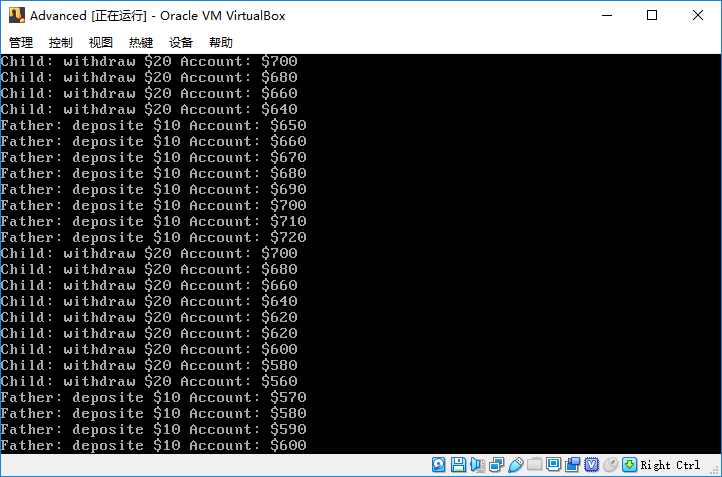
\includegraphics[width=0.8\linewidth]{fig/bank.PNG}\\
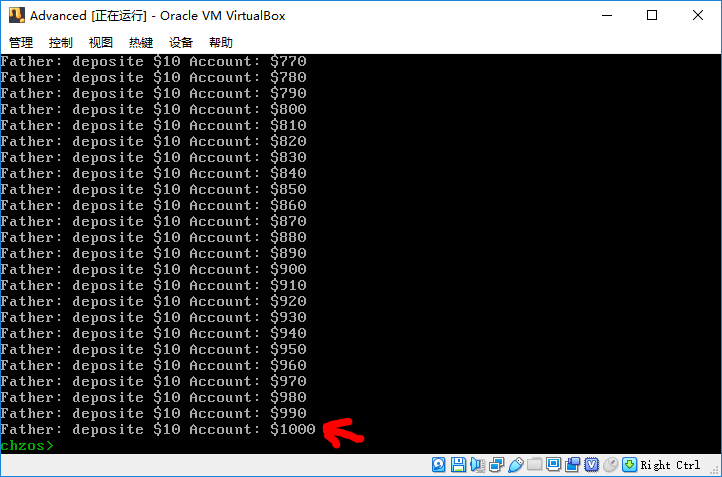
\includegraphics[width=0.8\linewidth]{fig/bank-final.PNG}
\end{tabular}
\caption{银行存取款结果}
\label{fig:bank}
\end{figure}

\subsection{父子祝福水果}
这是本实验要求中要完成的程序,代码如下。
儿子依次向父亲送上苹果、梨和香蕉,如此往复。

注意这里对老师课件上的程序进行了修改,\textbf{原程序是存在bug的!}
原程序中只使用了一个信号量,而这里我采用了四个信号量,以确保程序的正确性,具体原因下面会说明。
\begin{lstlisting}
#include "stdio.h"
#include "api.h"

enum FRUITS {
	NONE = 0,
	APPLE,
	PEAR,
	BANANA
} fruit_plate;

char words[100];
int fruit_index;

void put_words(char* w)
{
	strcpy(words,w);
}

void put_fruit()
{
	fruit_index = (fruit_index + 1) % 4;
	if (fruit_index == 0)
		fruit_index++;
	fruit_plate = fruit_index;
}

int sem_word, sem_fruit, sem_word_full, sem_fruit_full;

void main(){
	sem_word = get_sem(0);
	sem_fruit = get_sem(0);
	sem_word_full = get_sem(0);
	sem_fruit_full = get_sem(0);
	fruit_plate = fruit_index = 0;
	if (fork()){
		while(1){
			sem_wait(sem_word); // p0
			sem_wait(sem_fruit); // p1
			char fruit_name[10];
			if (fruit_plate == APPLE)
				strcpy(fruit_name,"APPLE");
			else if (fruit_plate == PEAR)
				strcpy(fruit_name,"PEAR");
			else if (fruit_plate == BANANA)
				strcpy(fruit_name,"BANANA");
			printf("%s %s!\n",words,fruit_name);
			sem_signal(sem_word_full); // v2
			fruit_plate = 0;
			sem_signal(sem_fruit_full); // v3
		}
	} else if (fork()) {
		while(1){
			put_words("Father will live forever!");
			sem_signal(sem_word); // v0
			sem_wait(sem_word_full); // p2
		}
	} else {
		while(1){
			put_fruit();
			sem_signal(sem_fruit); // v1
			sem_wait(sem_fruit_full); // p3
		}
	}
}
\end{lstlisting}

如果只采用一个信号量,即祝福和放水果都用同一个,这并无法保证父亲每次\textbf{恰好收到一份祝福和一个水果}时就输出,可能会出现两份祝福而没有水果,或两个水果而没有祝福的情况,因为这都符合信号量增加到0,取消阻塞的机制。

如果将祝福和放水果的信号量分离,即采用两个信号量,也同样是有问题的。
因为儿子并不知道父亲已经将祝福和水果拿走,因此在父亲没拿走这些物品之前,儿子就已经把新的放了上去,父亲拿走的时候就拿空了,下一次父亲就会以为儿子还没有放。
体现在程序中即父进程对\verb'words'和\verb'fruit_name'输出后,需要更新\verb'fruit_plate'为$0$,但在更新之前子进程实际上已经完成了\verb'put_fruit'操作,并且不断循环。
此时\verb'fruit_plate=0'覆盖掉了子进程放上去的水果,从而导致RC问题。
如图\ref{fig:fruit-wrong}所示,水果出现的次序并不是依照\verb'APPLE,PEAR,BANANA'这样,而更多是\verb'APPLE',这正是因为\verb'fruit_plate'被清空了,只能从$0$开始计数,进而导致意料之外的答案。

\begin{figure}[H]
\centering
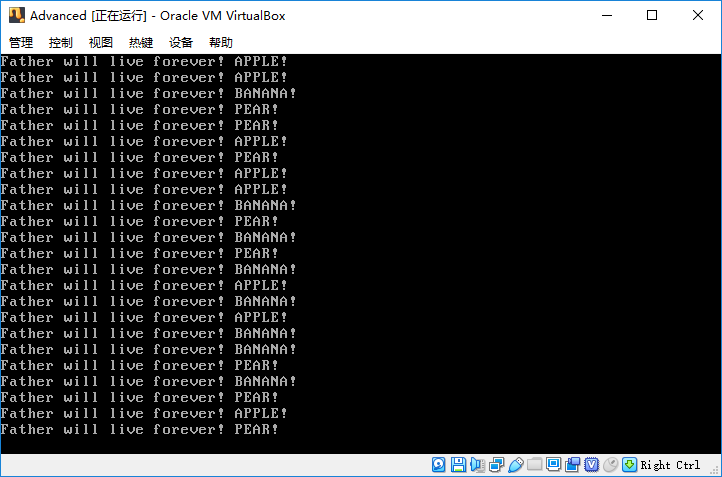
\includegraphics[width=0.8\linewidth]{fig/fruit-wrong.PNG}
\caption{祝福水果RC问题}
\label{fig:fruit-wrong}
\end{figure}

而正确的实现方式应该如我的代码所示,采用四个信号量。
\verb'sem_word'和\verb'sem_fruit'用来判断盘中是否有东西,儿子需要放了祝福或水果后父亲才能享用,这也是老师代码中所体现的。
但是老师的代码中忽视了还有另一个同步关系,即父亲享用完儿子才能放新的祝福或水果。
故需要\verb'sem_word_full'和\verb'sem_fruit_full'用来判断盘中是否满了,如果满了则不应该放置新的物品,防止新的东西被覆盖清除导致错误。

实验结果如图\ref{fig:fruit}所示,可以清晰地看到水果出现的次序严格依照\verb'APPLE,PEAR,BANANA'出现,解决了RC问题,确保了程序正确性。
\begin{figure}[H]
\centering
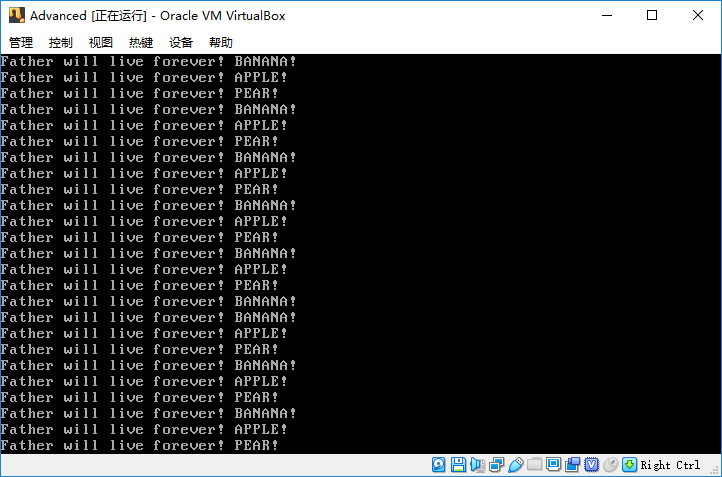
\includegraphics[width=0.8\linewidth]{fig/fruit.PNG}
\caption{祝福水果正确结果。注意由于动态截图的问题,故中间会出现两行同样的输出,但实际上这是输出太快而导致的截图暂留,原始输出结果是正确无误的!}
\label{fig:fruit}
\end{figure}

\subsection{生产者消费者模型}
本次实验还用信号量实现了生产者消费者模型,如下代码所示。
其中信号量\verb'mutex'用来保证互斥性,信号量\verb'n'用来保证同步关系。
\begin{lstlisting}
#include "stdio.h"
#include "api.h"

int tot;
int mutex;
int n;

void main() {
	tot = 0;
	mutex = get_sem(1);
	n = get_sem(0);
	int pid = fork();
	if (pid == -1) {
		printf("error in fork!");
		exit(-1);
	}
	if (pid) {
		while (1) { // Producer
			sem_wait(mutex);
			printf("Produce %d\n", ++tot);
			sem_signal(mutex);
			sem_signal(n);
		}
	} else {
		while (1) { // Consumer
			sem_wait(n);
			sem_wait(mutex);
			printf("Consume %d\n", tot--);
			sem_signal(mutex);
		}
	}
}
\end{lstlisting}

实验结果如图\ref{fig:ps}所示,可以看出只有生产者产生了某一序号的物品,消费者才会对其进行消费,如此持续。
\begin{figure}[H]
\centering
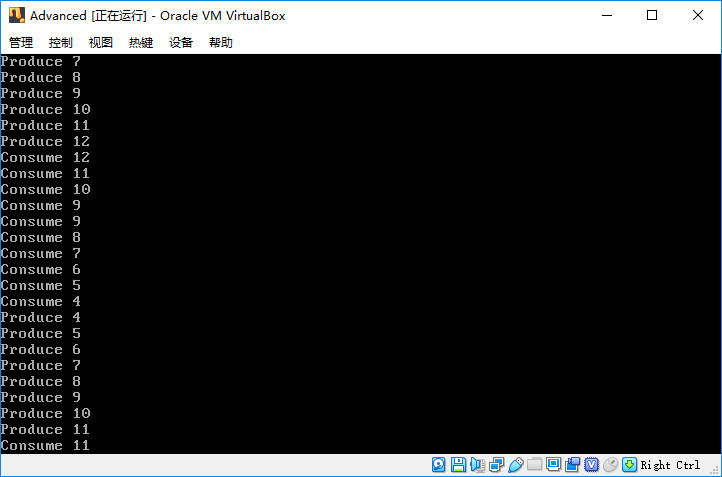
\includegraphics[width=0.8\linewidth]{fig/prod-cons.PNG}
\caption{生产者消费者模型结果。注意同样存在动态截图导致两行重复的问题,但结果是正确的!}
\label{fig:ps}
\end{figure}

同上一个祝福水果实验,实验结果都说明我的操作系统能够正确解决多进程、多信号量的情况,具有充分的灵活性和鲁棒性。

\section{实验总结}
% 每人必需写一段,文字不少于500字,可以写心得体会、问题讨论与思考、新的设想、感言总结或提出建议等等。不得抄袭,否则按作弊处理。
本次实验有了之前实验的基础,相对来讲比较简单,只需对照着信号量的原理,将四个基本操作实现一遍即可。

但实现过程中还是因为自己的疏忽出现了一些小问题。
如一开始以为信号量只需维护一个阻塞进程即可,在做银行存取款实验时没有出现任何问题,但到了父子祝福实验就始终做不对结果。
原因正是因为父子祝福实验涉及到三个进程,而仅仅维护一个阻塞进程就可能出现bug。
发现问题之后对相应的进程控制块进行修改,并在信号量操作中对阻塞队列进行维护,就可以确保在多进程环境下程序运行也不会出错了。

另一点则是在编写用户程序时的疏忽---误把信号量开为局部变量,导致信号量的值总是不如期望,逐行调试了很久才发现了这个问题。
不管是进程号、信号量、互斥锁等等,这些涉及到多进程协作的变量,就应该开设在全局,这样才有办法让各个进程共享使用,否则当新的进程产生后,它就不知道去哪里找对应的数据了,因为进程的克隆并没有拷贝所有的变量/内存内容。

总的来说,实现操作系统的时候还是应该更小心点。
对于操作系统来说,一个小的bug都很可能是致命的,这点尤为注意。

\section{参考资料}
\begin{enumerate}
	\item OS Development Series, \url{http://www.brokenthorn.com/Resources/OSDevIndex.html}
	\item Roll your own toy UNIX-clone OS, \url{http://www.jamesmolloy.co.uk/tutorial_html/}
	\item The little book about OS development, \url{http://littleosbook.github.io/}
	\item Writing a Simple Operating System from Scratch, \url{http://www.cs.bham.ac.uk/~exr/lectures/opsys/10_11/lectures/os-dev.pdf}
	\item Intel$^{\textregistered}$ 64 and IA-32 Architectures Software Developer's Manual
	\item UCore OS Lab, \url{https://github.com/chyyuu/ucore_os_lab}
	\item CMU CS 15-410, Operating System Design and Implementation, \url{https://www.cs.cmu.edu/~410/}
	\item 李忠,王晓波,余洁,《x86汇编语言-从实模式到保护模式》,电子工业出版社,2013
\end{enumerate}

\appendix
\appendixconfig
\section{程序清单}
\subsection{内核核心代码}
\begin{center}
\begin{tabular}{|c|l|l|}\hline
\textbf{序号} & \textbf{文件} & \textbf{描述} \\\hline
1 & \verb'bootloader.asm' & 主引导程序\\\hline
2 & \verb'kernel_entry.asm' & 内核汇编入口程序\\\hline
3 & \verb'kernel.c' & 内核C入口程序\\\hline
4 & \verb'Makefile' & 自动编译指令文件\\\hline
5 & \verb'bootflpy.img' & 引导程序/内核软盘\\\hline
6 & \verb'mydisk.hdd' & 虚拟硬盘\\\hline
7 & \verb'bochsrc.bxrc' & Bochs配置文件\\\hline
\end{tabular}
\end{center}

\subsection{内核头文件}
\begin{center}
\begin{tabular}{|c|l|l|}\hline
\textbf{序号} & \textbf{文件} & \textbf{描述} \\\hline
1 & \verb'disk_load.inc' & BIOS读取磁盘\\\hline
2 & \verb'show.inc' & 常用汇编字符显示\\\hline
3 & \verb'gdt.inc' & 汇编全局描述符表\\\hline
4 & \verb'gdt.h' & C全局描述符表\\\hline
5 & \verb'idt.h' & 中断描述符表\\\hline
6 & \verb'hal.h' & 硬件抽象层\\\hline
6.1 & \verb'pic.h' & 可编程中断控制器\\\hline
6.2 & \verb'pit.h' & 可编程区间计时器\\\hline
6.3 & \verb'keyboard.h' & 键盘处理\\\hline
6.4 & \verb'tss.h' & 任务状态段\\\hline
6.5 & \verb'ide.h' & 硬盘读取\\\hline
7 & \verb'io.h' & I/O编程\\\hline
8 & \verb'exception.h' & 异常处理\\\hline
9 & \verb'syscall.h' & 系统调用\\\hline
10 & \verb'task.h' & 多进程设施\\\hline
11 & \verb'user.h' & 用户程序处理\\\hline
12 & \verb'terminal.h' & Shell\\\hline
13 & \verb'scancode.h' & 扫描码\\\hline
14 & \verb'stdio.h' & 标准输入输出\\\hline
15 & \verb'string.h' & 字符串处理\\\hline
16 & \verb'elf.h' & ELF文件处理\\\hline
17 & \verb'api.h' & 进程管理API\\\hline
18 & \verb'semaphore.h' & 信号量机制\\\hline
\end{tabular}
\end{center}

\subsection{用户程序}
用户程序都放置在\verb'usr'文件夹中。
\begin{center}
\begin{tabular}{|c|l|l|}\hline
\textbf{序号} & \textbf{文件} & \textbf{描述} \\\hline
1-4 & \verb'prgX.asm' & 飞翔字符用户程序\\\hline
5 & \verb'box.asm' & 画框用户程序\\\hline
6 & \verb'sys_test.asm' & 系统中断测试\\\hline
7 & \verb'fork_test.c' & 进程分支测试\\\hline
8 & \verb'fork2.c' & 进程多分支测试\\\hline
9 & \verb'bank.c' & 银行存取款测试\\\hline
10 & \verb'fruit.c' & 父子祝福水果测试\\\hline
11 & \verb'prod_cons.c' & 消费者生产者模型测试\\\hline
\end{tabular}
\end{center}

\section{系统调用清单}
\label{sec:syscall}
\begin{center}
\begin{tabular}{|c|c|}\hline
\textbf{功能号} & \textbf{功能}\\\hline
0 & 输出OS Logo\\\hline
1 & 睡眠100ms\\\hline
10 & \verb'fork'\\\hline
11 & \verb'wait'\\\hline
12 & \verb'exit'\\\hline
13 & \verb'get_pid'\\\hline
20 & \verb'get_sem'\\\hline
21 & \verb'sem_wait'\\\hline
22 & \verb'sem_signal'\\\hline
23 & \verb'free_sem'\\\hline
100 & 返回内核Shell\\\hline
\end{tabular}
\end{center}

\end{document}

% 实验提交内容
% 实验报告:电子版(Word2003的DOC格式或PDF格式)
% 原程序文件及可执行代码程序文件
% 测试输入数据文件和输出数据文件
% 虚拟机软盘映像文件

% 基础实验项目5个和扩展实验7个
% 实验项目,迟交影响成绩评价!
% 工具与环境可由选择,开发新型工具或优化一套开发环境都可加分!
% 一系列基础实验项目必须连续完成,当前项目只能在前一个项目的基础上进行,体现出前后的进化关系,否则要被约谈,证明没有抄袭行为!
% 一个项目可提交多个改进的版本,实现新功能和个性化特征都有利于提高相应项目的成绩。
% 实验项目提交内容用winrar工具整体压缩打包,统一格式命名为:
%	<学号>+<姓名>+<实验项目号>+<版本号>.rar
%	姓名(学号)实验NvX.zip
%	实验报告、项目文件夹、映像文件
%	ftp://172.18.216.232 sysuac 下周六23:59

% 免考
% 条件:实验1~6全部评价AAAAB+B+或相当
% 最终成绩可能范围:75分以上